\documentclass{../../../oss-classkick}

\usepackage{circuitikz} % to draw circuits!
\usepackage{bm}

\begin{document}
\genheader

\genfreetitle{C}{MAGNETISM, HALL EFFECT AND MAXWELL'S EQUATIONS}{3}

% TAKEN FROM THE 2009 AP PHYSICS C FREE-RESPONSE QUESTION E&M 2. THIS IS A
% HALL-EFFECT QUESTION
\cpic{.45}{hall2}
\begin{enumerate}
\item A \SI{9.}{\volt} battery is connected to a rectangular bar of length
  \SI{0.080}{\metre}, uniform cross-sectional area \SI{5.0e-6}{\metre\squared},
  and resistivity \SI{4.5e-4}{\ohm.\metre}, as shown above. Electrons are the
  sole charge carriers in the bar. The wires have negligible resistance. The
  switch in the circuit is closed at time $t = 0$.
  \begin{enumerate}
  \item Calculate the power delivered to the circuit by the battery.
  \item On the diagram below, indicate the direction of the electric field in
    the bar.
    \begin{center}
      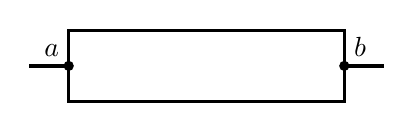
\begin{tikzpicture}[scale=.5]
        \draw[very thick](.5,.6) rectangle(7.5,2.4);
        \draw[very thick](-.5,1.5)--(.5,1.5);
        \draw[very thick](7.5,1.5)--(8.5,1.5);
        \fill(.5,1.5) circle(.13) node[above left] {$a$};
        \fill(7.5,1.5) circle(.13) node[above right]{$b$};
      \end{tikzpicture}

      Side View
    \end{center}
    Explain your answer.
  \item Calculate the strength of the electric field in the bar.
  \end{enumerate}
  A uniform magnetic field of magnitude \SI{.25}{\tesla} perpendicular to the
  bar is added to the region around the bar, as shown below.
  \cpic{.8}{hall1}
  \begin{enumerate}
  \item Calculate the magnetic force on the bar.
  \item The electrons moving through the bar are initially deflected by the
    external magnetic field. On the diagram below, indicate the direction of
    the additional electric field that is created in the bar by the deflected
    electrons.
    \begin{center}
      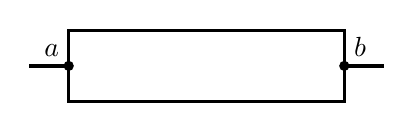
\begin{tikzpicture}[scale=.5]
        \draw[very thick](.5,.6) rectangle(7.5,2.4);
        \draw[very thick](-.5,1.5)--(.5,1.5);
        \draw[very thick](7.5,1.5)--(8.5,1.5);
        \fill(.5,1.5) circle(.13) node[above left] {$a$};
        \fill(7.5,1.5) circle(.13) node[above right]{$b$};
      \end{tikzpicture}

      Side View
    \end{center}
  \item The electrons eventually experience no deflection and move through the
    bar at an average speed of \SI{3.5e-3}{\metre\per\second}. Calculate the
    strength of the additional electric field indicated in part (e).
  \end{enumerate}
  \newpage

  % TAKEN FROM THE 2009 AP PHYSICS C EXAM FREE-RESPONSE QUESTION E&M 3
  % THIS IS A QUESTION ON MAGNETIC INDUCTION
  \begin{center}
    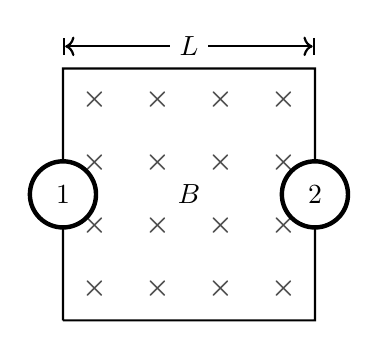
\begin{tikzpicture}[scale=.8]
      \foreach\x in {0,...,3}{
        \foreach\y in {0,...,3} \node[black!70] at (\x,\y){$\bm{\times}$};
      }
      \draw[thick](-.5,-.5) to[rmeter,t=1](-.5,3.5)--(3.5,3.5)
      to[rmeter,t=2] (3.5,-.5)--(-.5,-.5);
      \node at (1.5,1.5){$B$};
      \draw[thick,|<->|](-.5,3.85)--(3.5,3.85) node[midway,fill=white]{$L$};
    \end{tikzpicture}
  \end{center}
\item A square conducting loop of side $L$ contains two identical lightbulbs,
  1 and 2, as shown above. There is a magnetic field directed into the page in
  the region inside the loop with magnitude as a function of time $t$ given by
  $B(t)=at+b$, where $a$ and $b$ are positive constants. The lightbulbs each
  have constant resistance $R_0$. Express all answers in terms of the given
  quantities and fundamental constants.
  \begin{enumerate}
  \item Derive an expression for the magnitude of the emf generated in the loop.
  \item
    \begin{enumerate}
    \item Determine an expression for the current through bulb 2.
    \item Indicate on the diagram above the direction of the current through
      bulb 2.
    \end{enumerate}
  \item Derive an expression for the power dissipated in bulb 1.
  \end{enumerate}
  Another identical bulb 3 is now connected in parallel with bulb 2, but it is
  entirely outside the magnetic field, as shown below.
  \begin{center}
    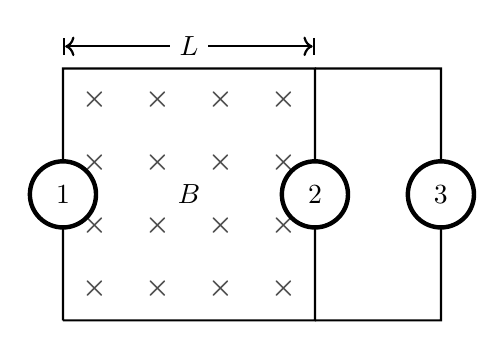
\begin{tikzpicture}[scale=.8]
      \foreach\x in {0,...,3}{
        \foreach\y in {0,...,3} \node[black!70] at (\x,\y){$\bm{\times}$};
      }
      \draw[thick](-.5,-.5) to[rmeter,t=1](-.5,3.5)--(3.5,3.5)
      to[rmeter,t=2] (3.5,-.5)--(-.5,-.5);
      \draw[thick](3.5,3.5)--(5.5,3.5) to[rmeter,t=3](5.5,-.5)--(3.5,-.5);
      \node at (1.5,1.5){$B$};
      \draw[thick,|<->|](-.5,3.85)--(3.5,3.85) node[midway,fill=white]{$L$};
    \end{tikzpicture}
  \end{center}
  \begin{enumerate}[resume]
  \item How does the brightness of bulb 1 compare to what it was in the
    previous circuit? Justify your answer.

    \vspace{.1in}
    \underline{\hspace{.4in}} Brighter\hspace{.5in}
    \underline{\hspace{.4in}} Dimmer\hspace{.5in}
    \underline{\hspace{.4in}} The same
  \end{enumerate}
  Now the portion of the circuit containing bulb 3 is removed, and a wire is
  added to connect the midpoints of the top and bottom of the original loop, as
  shown below.
   \begin{center}
    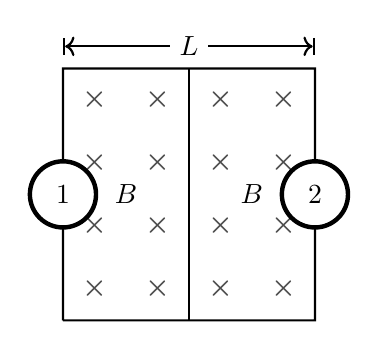
\begin{tikzpicture}[scale=.8]
      \foreach\x in {0,...,3}{
        \foreach\y in {0,...,3} \node[black!70] at (\x,\y){$\bm{\times}$};
      }
      \draw[thick](-.5,-.5) to[rmeter,t=1](-.5,3.5)--(3.5,3.5)
      to[rmeter,t=2] (3.5,-.5)--(-.5,-.5);
      \draw[thick](1.5,3.5)--(1.5,-.5);
      \node at (.5,1.5){$B$};
      \node at (2.5,1.5){$B$};
      \draw[thick,|<->|](-.5,3.85)--(3.5,3.85) node[midway,fill=white]{$L$};
    \end{tikzpicture}
  \end{center}
  \begin{enumerate}[resume]
  \item How does the brightness of bulb 1 compare to what it was in the first
    circuit? Justify your answer.

    \vspace{.1in}
    \underline{\hspace{.4in}} Brighter\hspace{.5in}
    \underline{\hspace{.4in}} Dimmer\hspace{.5in}
    \underline{\hspace{.4in}} The same
  \end{enumerate}
  \newpage

  \begin{center}
    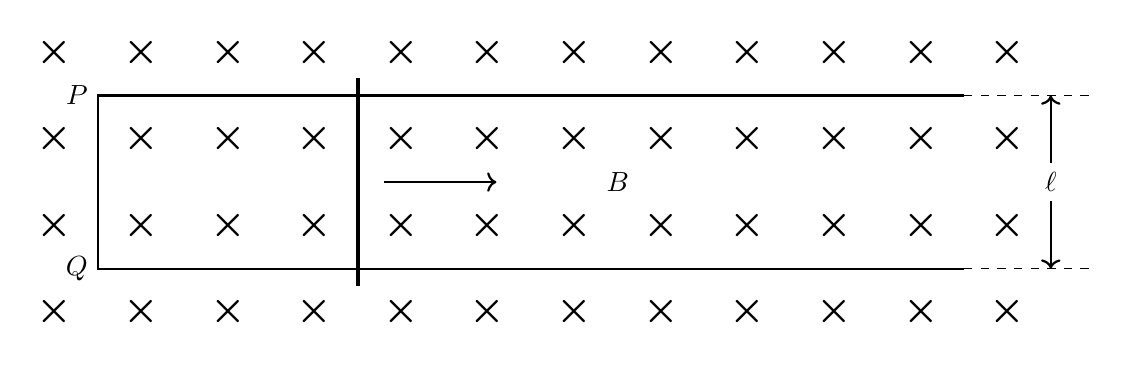
\begin{tikzpicture}[scale=1.1]
      \foreach \x in {0,...,11}
      \foreach \y in {0,...,3} \node at (\x,\y) {\Large$\bm{\times}$};
      \draw[thick](10.5,.5)--(.5,.5) node[left]{$Q$}--(.5,2.5) node[left]{$P$}
      --(10.5,2.5);
      \draw[dashed](10.5,2.5)--(12,2.5);
      \draw[dashed](10.5,0.5)--(12,0.5);
      \draw[ultra thick](3.5,.3)--(3.5,2.7);
      \node at (6.5,1.5) {$B$};
      \draw[thick,<->](11.5,.5)--(11.5,2.5) node[midway,fill=white]{$\ell$};
      \draw[thick,->](3.8,1.5)--(5.1,1.5) node[midway,above]{$\varv$};
    \end{tikzpicture}

    Top View
  \end{center}
\item In the diagram above, a nichrome wire of resistance per unit length
  $\lambda$ is bent at points $P$ and $Q$ to form horizontal conducting rails
  that are a distance $\ell$ apart. The wire is placed within a uniform
  magnetic field of magnitude $B$ pointing into the page. A conducting rod of
  negligible resistance, which was aligned with end $PQ$ at time $t=0$, slides
  to the right with constant speed $\varv$ and negligible friction. Express all
  algebraic answers in terms of the given quantities and fundamental constants.
  \begin{enumerate}
  \item Indicate the direction of the current induced in the circuit. Justify
    your answer.

    \vspace{.1in}
    \underline{\hspace{.4in}} Clockwise\hspace{.5in}
    \underline{\hspace{.4in}} Counterclockwise

  \item Derive an expression for the magnitude of the induced current as a
    function of time $t$.
  \item Derive an expression for the magnitude of the magnetic force on the rod
    as a function of time.
  \item On the axes below, sketch a graph of the external force $F_\text{ext}$
    as a function of time that must be applied to the rod to keep it moving at
    constant speed while in the field. Label the values of any intercepts.
    \begin{center}
      \begin{tikzpicture}
        \draw[very thick,->](0,0)--(7,0) node[right]{$t$}
        node[pos=0,below left]{$O$};
        \draw[very thick,->](0,0)--(0,4) node[above]{$F_\text{ext}$};
      \end{tikzpicture}
    \end{center}
  \item The force pulling the rod is now removed. Indicate whether the speed of
    the rod increases, decreases, or remains the same. Justify your answer.

    \vspace{.1in}
    \underline{\hspace{.4in}} Increases\hspace{.5in}
    \underline{\hspace{.4in}} Decreases\hspace{.5in}
    \underline{\hspace{.4in}} Remains the same
  \end{enumerate}
\end{enumerate}
\end{document}
